%%%%%%%%%%%%%%%%%%%%%%%%%%%%%%%%%%%%%%%%%%%%%%%%%%%%%%%%%
% SOUBOR: README.tex
% AUTOR: Drahomir Dlabaja (xdlaba02)
% DATUM: 23. 4. 2020
%%%%%%%%%%%%%%%%%%%%%%%%%%%%%%%%%%%%%%%%%%%%%%%%%%%%%%%%%

\documentclass[a4paper, 11pt, titlepage]{article}

\usepackage[total={17cm,25cm}, top=3cm, left=2cm, includefoot]{geometry}
\usepackage[czech]{babel}
\usepackage[utf8]{inputenc}
\usepackage{graphicx}
\usepackage{hyperref}
\usepackage{multirow}

\usepackage{etoolbox}
\preto\tabular{\shorthandoff{-}}

\begin{document}
	\begin{centering}
		\Large\textsc{Multimédia}\\[1em]
		\Huge{Bezeztrátová komprese obrazu}\\[1em]
		\Large{Drahomír Dlabaja (xdlaba02)}\\
		\today\\
	\end{centering}

	\section*{Zadání}

	\begin{itemize}
	 \item Seznamte se s~metodami bezeztrátové komprese obrazu (predikce, kódování rozdílu, entropické kódování).
   \item Navrhněte a~implementujte postup komprese obrazu s~použitím vybraných metod.
   \item Porovnejte dosaženou účinnost komprese se v~současnosti používanými formáty (PNG).
	\end{itemize}

	\section*{Řešení}
  Řešení tohoto projektu je částečně sdílené s~řešením projektu do předmětu Kódování a~komprese dat.
	Projekt obsahuje částečně shodné zdrojové kódy implementace jednotlivých metod komprese, avšak kompresní řetězec jako takový se liší.
	Řešení využívá zdrojové kódy z~knihovny \texttt{liblfif}\footnote{\url{https://github.com/xdlaba02/light-field-image-format/tree/master/liblfif}} a~k ní příslušejících nástrojů.
	Dále řešení používá celou knihovnu \texttt{libppm}\footnote{\url{https://github.com/xdlaba02/light-field-image-format/tree/master/libppm}} pro čtení a~zápis PPM souborů.
	Byla využita knihovna \texttt{libdivsufsort}\footnote{\url{https://github.com/y-256/libdivsufsort}}, která efektivně implementuje Burrows-Wheelerovu transformaci.

	První část kompresního řetězce je inspirována metodou \texttt{PNG}, ze které si vypůjčuje Paethův prediktor. Ten je však modifikován pro přirozené obrázky.
	Druhá část je založená na bezeztrátové kompresní metodě \texttt{bzip2}, ze které je vypůjčena Burrows-Wheelerova transformace v~kombinaci s~Move-to-front transformací.
	Takto zpracovaná data jsou entropicky kódována kontextově-adaptivním binárním aritmetickým kodérem \texttt{CABAC}.

	\subsection*{Subtract Green Transformace\footnote{\url{https://developers.google.com/speed/webp/docs/compression}}}
	Prvním krokem komprese je dekorelace barevných složek.
	K tomuto účelu existují barevné prostory, které oddělují jas od barevné složky (YCbCr, YCoCg).
	Tyto prostory jsou hojně používané ve ztrátové kompresi, která využívá toho, že lidské oko je méně citlivé na chromaticitu než na jas.
	Jelikož tento projekt řeší bezeztrátovou kompresi, nedají se tyto prostory využít, protože pro přesnou reprezentaci barev v~těchto prostorech je potřeba více bitů, než by bylo pro kompresi praktické.

	Pro dekorelaci barev byla v~tomto projektu využita transformace odečtení zelené.
	Ta spočívá pouze v~tom, že od hodnot červené a~modré se odečte zelená složka.
	V důsledku to znamená, že trojice $(R, G, B)$ se převede na $(R - G, G, B - G)$.
	Tato transformace vychází z~toho, hodnota zelené složky je velmi podobná hodnotě jasu, a~je tedy korelovaná s~hodnotami červené a~modré.
	Tato transformace barev je výhodná v~tom, že je bezeztrátová.
	Na straně dekodéru se pouze přičte zelená složka ke zbylým hodnotám a~vznikne původní trojice $(R,G,B)$.
	Pokud jsou vstupní data na osmi bitech, lze výstup této transformace reprezentovat opět na osmi bitech pomocí operace modulo.
	To sice může způsobit velké skoky mezi hodnotami sousedících vzorků, ale s~tím se vypořádají následující kroky komprese.

	\subsection*{Modifikovaný Paethův prediktor\footnote{\url{https://www.w3.org/TR/PNG-Filters.html}}}
	Formát \texttt{PNG} využívá ke kompresi řadu predikčních filtrů.
	Použitý filtr je zvolen pro každý řádek obrazu a~pro každý barevný kanál.
	Kodér má tak možnost v~závislosti na požadované rychlosti vyzkoušet více či méně kombinací a~dosáhnout tak lepší či horší komprese.

	Filtr \textit{NONE} ponechává aktuální hodnotu vzorku beze změny.
	Filtr \textit{SUB} od aktuální hodnoty vzorku odečte hodnotu vzorku, který se nachází bezprostředně před tímto vzorkem.
	Filtr \textit{UP} od aktuální hodnoty vzorku odečte hodnotu vzorku, který se nachází bezprostředně nad tímto vzorkem.
	Filtr \textit{AVG} od aktuální hodnoty vzorku odečte průměr z~hodnot vzorků, které se nachází bezprostředně před a~nad tímto vzorkem.
	Filtr \textit{PAETH} nejdříve vypočte lineární funkci z~bezprostředně před\-chá\-ze\-jí\-cí\-ho levého, horního a~levého horního vzorku.
	Poté od aktuální hodnoty vzorku odečte souseda s~nejmenším rozdílem od funční hodnoty zmíněné lineární funkce.

	Experimentálně bylo zjištěno, že predikce dosahuje poměrně dobrých výsledků při použití samo\-stat\-né\-ho Paethova prediktoru pro celý obrázek.
	Pomine tak nutnost pro každý řádek zapisovat, který prediktor byl použit.
	Původní Paethův prediktor předpokládal, že aktuální vzorek bude mít stejnou barvu jako jeden ze sousedních.
	To je pravdivé pro ilustrované obrázky s~ostrými přechody, avšak přirozené obrázky obsahují plynulé přechody, proto byla do prediktoru přidána možnost volby predikce z~průměru sousedních vzorků.
	Experimenty ukázaly, že tato modifikace zlepšuje kompresní výkon.

	\subsection*{Burrows-Wheelerova transformace}
	Burrows-Wheelerova transformace přeuspořádá vstupní řetězec na jednu z~jeho permutací tak, aby se podobné symboly nacházely s~velkou prav\-dě\-po\-dob\-nos\-tí blízko sebe.
	Tato transformace je bezeztrátově reverzibilní, pro inverzní transformaci je potřeba pouze index permutace, která byla použita.
	V tomto projektu byla pro Burrows-Wheelerovu transformaci použita knihovna \texttt{libdivsufsort}, která ji implementuje s~lineární časovou složitostí pomocí pole suffixů.

	Metoda \texttt{bzip2} provádí před Burrows-Wheelerovou transformací ještě kódování délek sledů bez explicitní značky.
	Experimentálně bylo zjištěno, že kódování délek sledů nepřináší žádný užitek, snad kromě mírného zkrácení doby Burrows-Wheelerovy transformace.
	Kódování délek sledů bylo z~tohoto důvodu v~tomto projektu vypuštěno.

	\subsection*{Move-to-front transformace}
	Move-to-front transformace začíná s~libovolně seřazeným -- avšak stejným na straně kodéru i~dekodéru -- seznamem kódovaných symbolů.
	Kódování jednoho symbolu zahrnuje vyhledání symbolu v~seznamu.
	Zakódovaný symbol je hodnota pořadí v~tomto seznamu.
	Seznam se poté aktualizuje přesunem kódovaného symbolu na jednu z~vyšších příček.

	Metoda aktualizace seznamu určuje efektivitu transformace pro daný zdroj.
	Základní verze aktualizace přesune zakódovaný symbol na první místo v~seznamu.
	To má za následek, že symbol se velmi snadno dostane na první místo.
	Alternativně existuje \textit{sticky} varianta Move-to-front transformace, která zakódovaný symbol přesune na určité procento svého původního pořadí.

	Vstupem tohoto kroku jsou data z~Burrows-Wheelerovy transformace.
	Podobné symboly se nacházejí s~velkou prav\-dě\-po\-dob\-nos\-tí blízko sebe.
	Move-to-front transformace z~takového zdroje vyprodukuje s~velikou pravděpodobností sekvenci, ve které se budou nacházet malá čísla.
	Experimentálně bylo zjištěno, že pro tento zdroj dosahuje dobrých výsledků \textit{sticky} varianta s~koeficinetem $c = 0.9$, tedy symbol se přesune na 90 \% svého původního pořadí.

	\subsection*{Kontextově-adaptivní binární aritmetické kódování}
	Posledním krokem kódování symbolů, kdy probíhá samotná komprese, je kontextově-adaptivní binární aritmetické kódování.
	Aritmetické kódování dokáže reprezentovat symbol na necelém počtu bitů a~mnohem lépe tak aproximuje entropii zdroje.
	Binární aritmetické kódování dokáže kódovat pouze binární hodnoty, avšak profituje z~velmi jednoduché implementace.
	Uživatel má v~tomto případě možnost kódovaná data binarizovat podle své potřeby a~není omezen pevnou délkou symbolu.
	Kontextové aritmetické kódování umožňuje uživateli volit rozložení pravděpodobnosti výskytu symbolů v~závislosti na již zakódovaných datech, nejčastěji podle symbolů bezprostředně před\-chá\-ze\-jí\-cí\-ch právě kódovanému symbolu.
	Tímto způsobem lze aproximovat entropii libovolného řádu a~využít tak všech známých vlastností zdroje.
	Adaptivní kódování pracuje pouze v~jednom průchodu. Po zakódování symbolu se aktualizuje rozložení pravděpodobností v~použitém kontextu.
	Kontexty jsou voleny a~aktualizovány deterministicky z~dat, které jsou již dostupné dekodéru.
	Na výstup není potřeba zapisovat model dat.

	V tomto projektu bylo použito 255 kontextů. Každý symbol byl binarizován pomocí unárního kódování a~k zakódování $n$-té binární hodnoty byl využit $n$-tý kontext.
	Číslo $k$ je unárně reprezentováno sekvencí $k$ jedniček ukončenou jednou nulou. Toto neplatí pro hodnotu 255, která ukončena nulou není.
	Na straně dekodéru se předpokládá, že na vstupu nebude větší hodnoty než 255.
	Počet binárních kontextů byl zvolen tak, aby simuloval jeden 8bitový kontext, který ukládá rozložení prav\-dě\-po\-dob\-nos\-tí pro 256 symbolů.
	To znamená, že z~hlediska symbolů je aproximována pouze entropie nultého řádu.

	Implementace kodéru umožňuje zapisovat data pomocí bypass módu, který nepracuje s~kontextem a~předpokládá uniformní rozložení kódovaných symbolů.
	Pomocí tohoto módu jsou na výstup zapsány metadata pro dekompresi, jako je rozlišení obrázku a~index permutace z~Burrows-Wheelerovy transformace.
	Výhodou tohoto přístupu je pozbytí nutnosti terminovat aktuální běžící aritmetický kodér.

	\section*{Implementace}
	Zdrojové kódy implementace kompresního řetězce se nachází v~podsložce \texttt{src}.
	Program je členěn do logických modulů:
	\begin{itemize}
		\item \textbf{bitstream} -- Čtení a~zápis po jednotlivých bitech zapouzdřující C++ streamy.
		\item \textbf{bwt} -- Zapouzdření knihovny \texttt{libdivsufsort}.
		\item \textbf{cabac} -- Implementace Kontextově-adaptivního binárního aritmetického kódování, vypůjčeno z~knihovny \texttt{liblfif}.
		\item \textbf{main} -- Zpracování parametrů příkazové řádky, samotné kompresní a~dekompresní řetězce.
		\item \textbf{mtf} -- Implementace různých variant move-to-front transformace.
		\item \textbf{predict} -- Implementace prediktorů.
	\end{itemize}

	\section*{Překlad a~použití}
	Zdrojové kódy lze přeložit pomocí příkazu \texttt{make} v~kořenové složce projektu.
	Pro kompresi \texttt{ppm} souboru lze nástroj volat takto:
	\begin{verbatim}
		./MUL_codec -i <ifile>.ppm -o <ofile>.mul -c
	\end{verbatim}
	Pro dekompresi lze nástroj volat podobně:
	\begin{verbatim}
		./MUL_codec -i <ifile>.mul -o <ofile>.ppm -d
	\end{verbatim}

  \section*{Vyhodnocení}
	Kodek byl vyhodnocen na datasetu veřejně dostupných light-field obrázků.
	Z každého obrázku byl vybrán prostřední pohled.
	Tento dataset byl využit z důvodu snadné dostupnosti na autorově zařízení.
	Kodek byl srovnán se třemi běžně používanými formáty pro bezeztrátovou kompresi obrazu.
	\begin{itemize}
		\item JPEG 2000, který je založený na bezeztrátové vlnkové transformaci,
		\item PNG, který je na webu hojně rozšířený a
		\item WEBP z dílny společnosti Google.
	\end{itemize}

	Pro každý obrázek a kodek byl měřen kompresní poměr, čas komprese a čas dekomprese.
	Obrázky byly komprimovány a dekomprimovány pomocí nástrojů z rodiny ImageMagick.
	V~grafech \ref{fig:bitrate}, \ref{fig:compress} a~\ref{fig:decompress} jsou vizualizovány výsledky srovnání.
	Kodek tohoto projektu je reprezentován zkratkou MUL.

	Z naměřených dat plyne, že implementovaný kodek dosahuje srovnatelného kompresního poměru v porovnání s ostatními kodeky.
	Ve většině případu kodek překonává metodu PNG, v některých případech dokonce i JPEG 2000.
	Z testovaných kodeků dosahuje nejlepší komprese metoda WEBP.

	Z hlediska doby komprese je navržený kodek ve většině případů rychlejší než WEBP a PNG.
	Z hlediska doby dekomprese je navržený kodek ve všech případech nejpomalejší.
	Z dat plyne, že metoda WEBP je asymetrická, z pohledu doby dekomprese se ukazuje jako nejrychlejší z testovaných metod.
	Metoda PNG dekomprimuje srovnatelně rychle v porovnání s WEBP.

	\begin{figure}[h!]
	\centering
	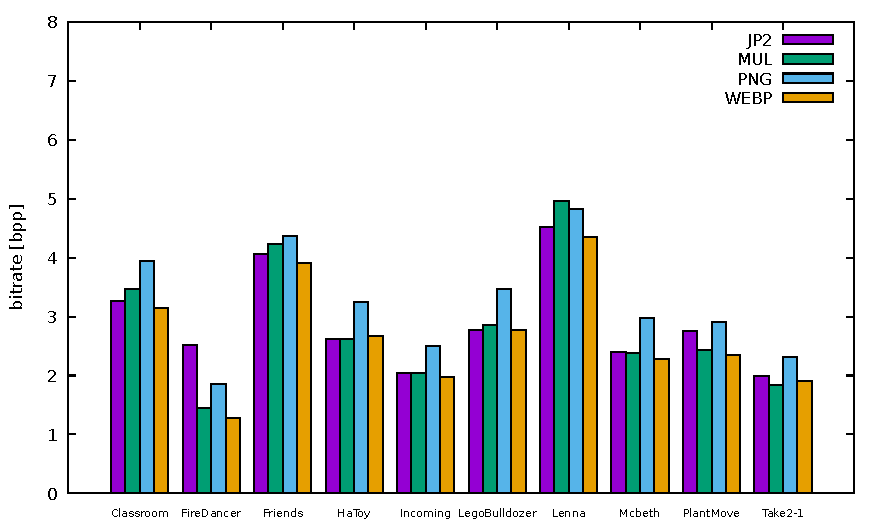
\includegraphics[width=15cm]{bitrate.pdf}
	\caption{Histogram datových toků.}
	\label{fig:bitrate}
	\end{figure}

	\begin{figure}[h!]
	\centering
	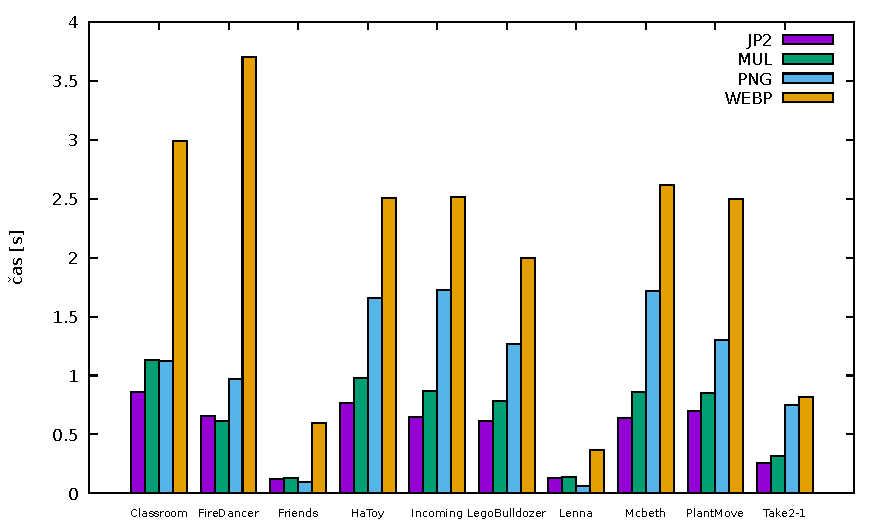
\includegraphics[width=15cm]{compress_time.pdf}
	\caption{Histogram doby komprese.}
	\label{fig:compress}
	\end{figure}

	\begin{figure}[h!]
	\centering
	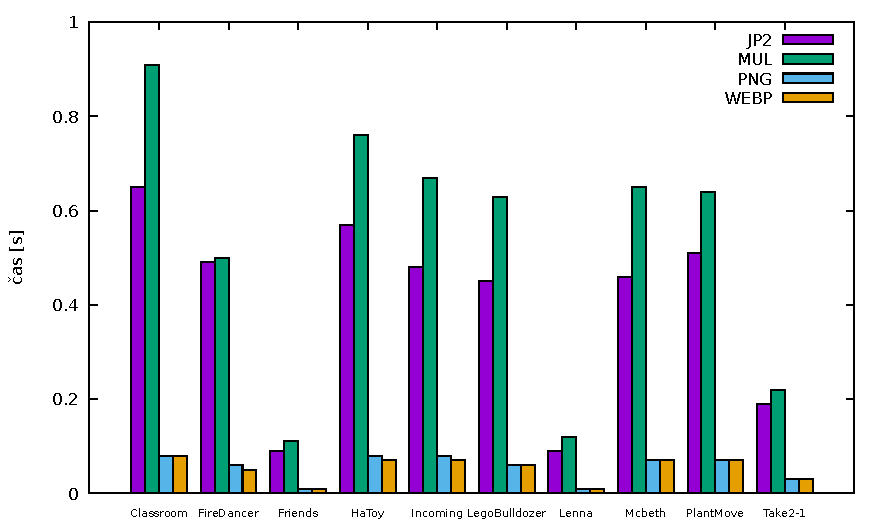
\includegraphics[width=15cm]{decompress_time.pdf}
	\caption{Histogram doby dekomprese.}
	\label{fig:decompress}
	\end{figure}

\end{document}
